%-------------------------------------------------------------------------------------------
	\section{Introduction}
%-------------------------------------------------------------------------------------------

An RNA sequence, over nucleotides of four kinds {\tt A}, {\tt C}, {\tt G}, {\tt U}, is synthesized (\textit{transcribed}) from its template DNA sequence over {\tt A}, {\tt C}, {\tt G}, {\tt T} nucleotide by nucleotide by an RNA polymerase (RNAP) enzyme according to the one-to-one mapping ${\tt A} \to {\tt U}$, ${\tt C} \to {\tt G}$, ${\tt G} \to {\tt C}$, and ${\tt T} \to {\tt A}$ (for details, see, e.g., \cite{AJLMRRW2014}). 
The yield, called \textit{transcript}, starts folding immediately after it emerges from RNAP. 
This is the \textit{cotranscriptional folding} (see Fig.~\ref{fig:rna_origami}). 
Geary, Rothemund, and Andersen have recently demonstrated the capability of cotranscriptional folding to self-assemble an RNA molecule of an intended shape at nano-scale \cite{GearyRothemundAndersen2014}. 
They actually proposed an architecture of a DNA sequence whose transcript folds cotranscriptionally into an RNA tile of specific rectangular shape highly likely \textit{in vitro}. 

\begin{figure}[tb]
\centering
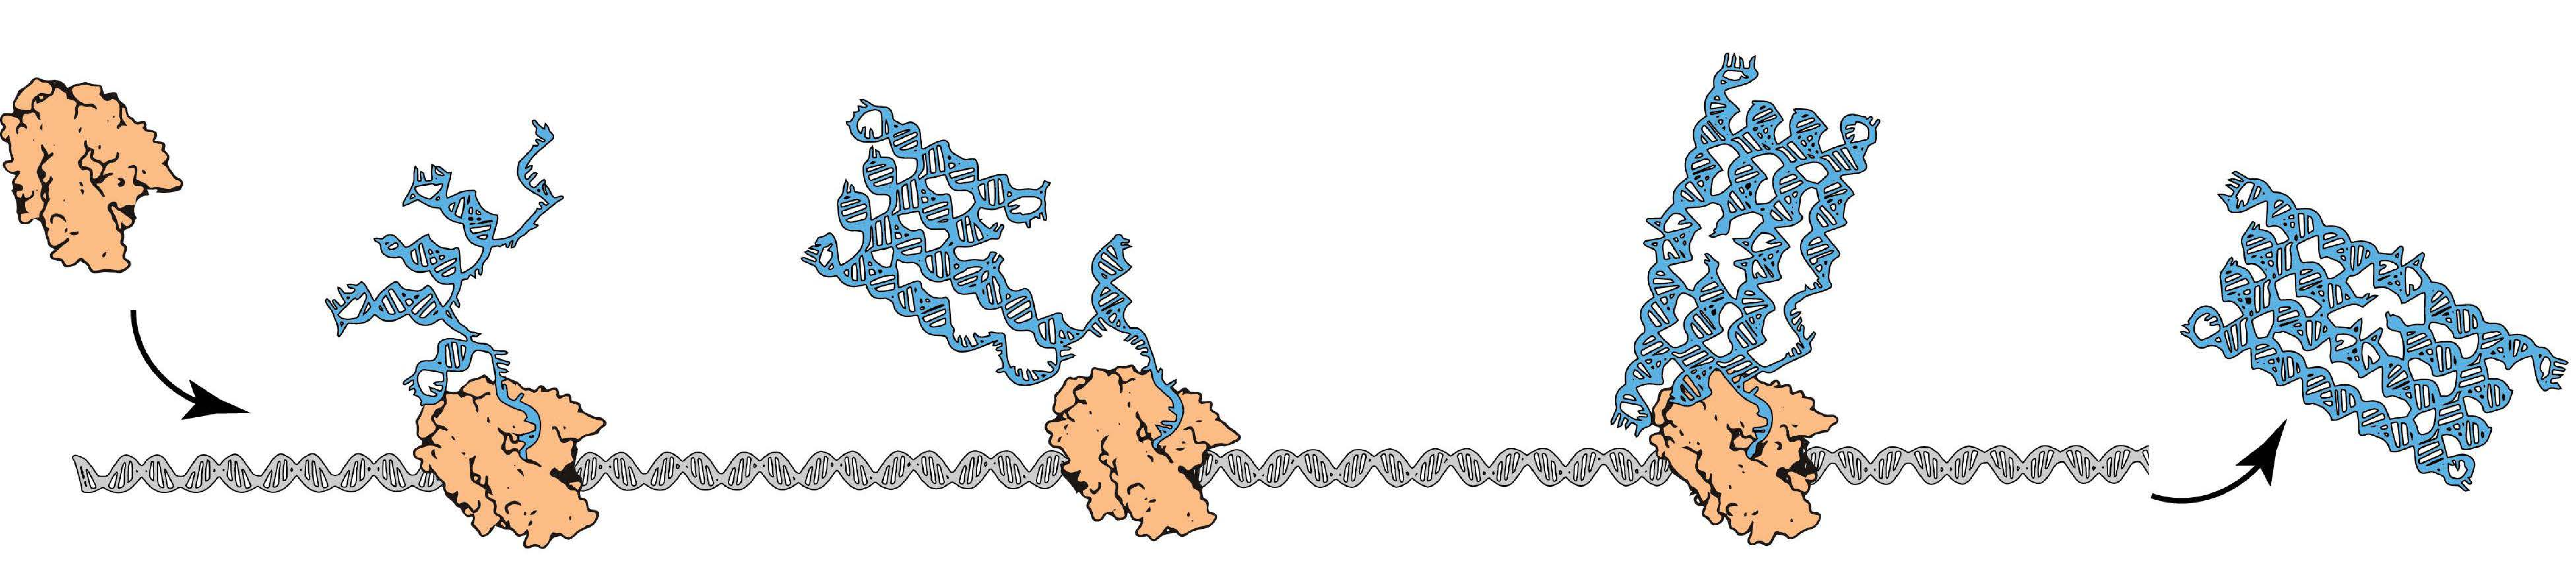
\includegraphics[width=0.8\linewidth]{pic/rna_origami.pdf}
\caption{RNA cotranscriptional folding. 
An RNA polymerase attaches to a template DNA sequence (gray spiral), scans it through, and synthesizes its RNA copy. 
The RNA sequence begins to fold upon itself immediately as it emerges from polymerase. 
}
\label{fig:rna_origami}
\end{figure}

%In this paper, we shall initiate the theoretical study on algorithmic self-assembly of shapes by cotranscriptional folding using a novel computational model of cotranscriptional folding called the \textit{oritatami system} \cite{GeMeScSe2016}.
Algorithms and computation are fundamental to molecular self-assembly as illustrated in an enormous success of their use in DNA tile self-assembly (see, e.g., \cite{Doty2012,Patitz2016,WinfreePhD} and references therein). 
%The concepts of computation and algorithms are yet to be as much utilized in the self-assembly of shapes by cotranscriptional folding as in the DNA tile self-assembly, where for example 
The Sierpinski triangle fractal was algorithmically self-assembled even \textit{in vitro} from coalescence of DNA tiles that compute XOR \cite{RothemundPapadakisWinfree2004}. 
Cotranscriptional folding exhibits highly sophisticated computational and algorithmic behaviors as well. 
Indeed, fluoride riboswitches in \textit{Bacillus cereus} bacteria cotranscriptionally fold into a terminator stem or does not in order to regulate gene expression \cite{WaStYuLiLu2016}. %depending on ligand concentration \cite{WaStYuLiLu2016}. 
This is just one example but should be enough to signify the context-sensitivity of cotranscriptional folding and shapes thus self-assembled. 
Geary et al.~have proved the capability of context-sensitivity to count in binary using a novel mathematical model of cotranscriptional folding called \textit{oritatami system} (abbreviated as OS) \cite{GeMeScSe2016}. 

%Cotranscriptional folding is in fact proved Turing-universal by the oritatami system \cite{GeMeScSe2015}. 
%The Turing-machine simulator is gigantic and intricate but oritatami systems have implemented basic computational devices such as binary counter \cite{GeMeScSe2016} as a module comparable in size to the gene expression regulator. 
%The binary counter module consists of half-adder components, which fold into one of possible four conformations depending on a 1-bit input and a 1-bit carry/non-carry encoded in their surroundings somehow. 
%It can be diverted as a copier for binary sequences by being fed with the non-carry. 
%They shall be reused in this paper. 

\begin{figure}[tb]
\centering
\begin{minipage}{0.4\linewidth}
\centering
\scalebox{0.7}{\begin{tikzpicture}[>=latex, node distance=2cm, initial text=, bend angle=15]
	\tikzstyle{every initial by arrow} = [->, double];

	\node [state, initial] (q_0)                        {$q_0/R$};
	\node [state]                     (q_1) [right of = q_0]  {$q_1/R$};
	\node [state]                     (q_2) [below right of = q_1] {$q_2/L$};
	\node [state]                     (q_3) [above right of = q_1] {$q_3/R$};

	\path [->] (q_0) edge [right] node [above]              {$0$}                 (q_1)
         		         edge [loop above] node [above]             {$1$}               ()
         			   (q_1) edge [bend left] node [above]             {$0$}                 (q_3)
         		         edge [bend right] node [below]             {$1$}              (q_2)
         			   (q_2)  edge [loop above] node [above]             {$0,1$}               ()
         			   (q_3)  edge [loop above] node [above]             {$0,1$}               ();
\end{tikzpicture}}
\end{minipage}
\begin{minipage}{0.05\linewidth}
\ \\
\end{minipage}
\begin{minipage}{0.5\linewidth}
\centering
\scalebox{0.03}{\begin{tikzpicture}
  \draw[blue!50!black,rotate=270,l-system={rule set={X->X-YF,Y->FX+Y},
  step=100pt,angle=90,axiom=FX,order=10},-triangle 90] l-system;
\end{tikzpicture}}
\end{minipage}
\caption{
%Heighway dragon. 
(Left) DFAO to output the direction (L/R) of $i$-th turn of the Heighway dragon given $i \ge 0$ in binary from the LSB. 
(Right) The first $2^{10}{-}1$ turns of the dragon. 
}
\label{fig:heighway_dragon}
\end{figure}

We shall initiate theoretical study on algorithmic self-assembly of shapes by cotranscriptional folding using oritatami system. 
Sierpinski triangle would allow our study to borrow rich insights from the DNA tile self-assembly. 
However, in order to cut directly to the heart of algorithmic self-assembly by cotranscriptional folding, shapes of choice should be traversable somehow algorithmically. 
One such way is to feed a turtle program (see \cite{AbelsondiSessa1981}) with an \textit{automatic sequence} as commands (drawing a line segment, rotation, etc.), whose $i$-th bit can be obtained by giving $i$ in binary from the least significant bit (LSB) to one DFA with output (DFAO) \cite{AlloucheShallit2003}.
Shapes thus describable include the Heighway dragon \cite{AlloucheShallit2003} and von Koch curve \cite{MaHoldener2005}. 
A DFAO for the Heighway dragon (Fig.~\ref{fig:heighway_dragon}) outputs the following sequence, given $i = 0, 1, 2, \ldots$ in binary: 
%It is to read the binary representation of $i \ge 0$ from the LSB and outputs the $i$-th direction $P[i]$ to turn (L or R) assigned to the state finally reached as follows: 
\[
%\begin{array}{cccrrrrc}
%i 	&=& 0 &  2 & 6 & 14 & 30 & \cdots \\
%P[i] 	&=& {\rm R} & {\rm RL} & {\rm RRLL} & {\rm RRRLLRLL} & {\rm RRRLRRLLLRRLLRLL} & \cdots.
%\end{array}
P 	= {\rm RRLRRLLRRRLLRLLRRRLRRLLLRRLLRLL} \cdots.
\]
(The notation $P$ is after its appellative \textit{paperfolding sequence} \cite{AlloucheShallit2003}.) 
For instance, $i = 2$ is given in binary from the LSB as 01, with which the DFAO transitions as $q_0 \to q_1 \to q_2$ and hence $P[2] = L$. 
%where only the values of $i$ at the end of the first five iterations are specified. 
A turtle should interpret an L (resp.~R) as ``move forward by unit distance and turn left (resp. right) 90 degrees.''
Any portion of the dragon can be represented by a factor of $P$; for instance, Fig.~\ref{fig:heighway_dragon} (Right) depicts the factor $P[0 .. 1022]$, i.e., the first $2^{10}-1$ turns of the dragon. 

%\begin{figure}[htb]
\begin{wrapfigure}{l}{0.57\linewidth}
\vspace*{-5mm}
\centering
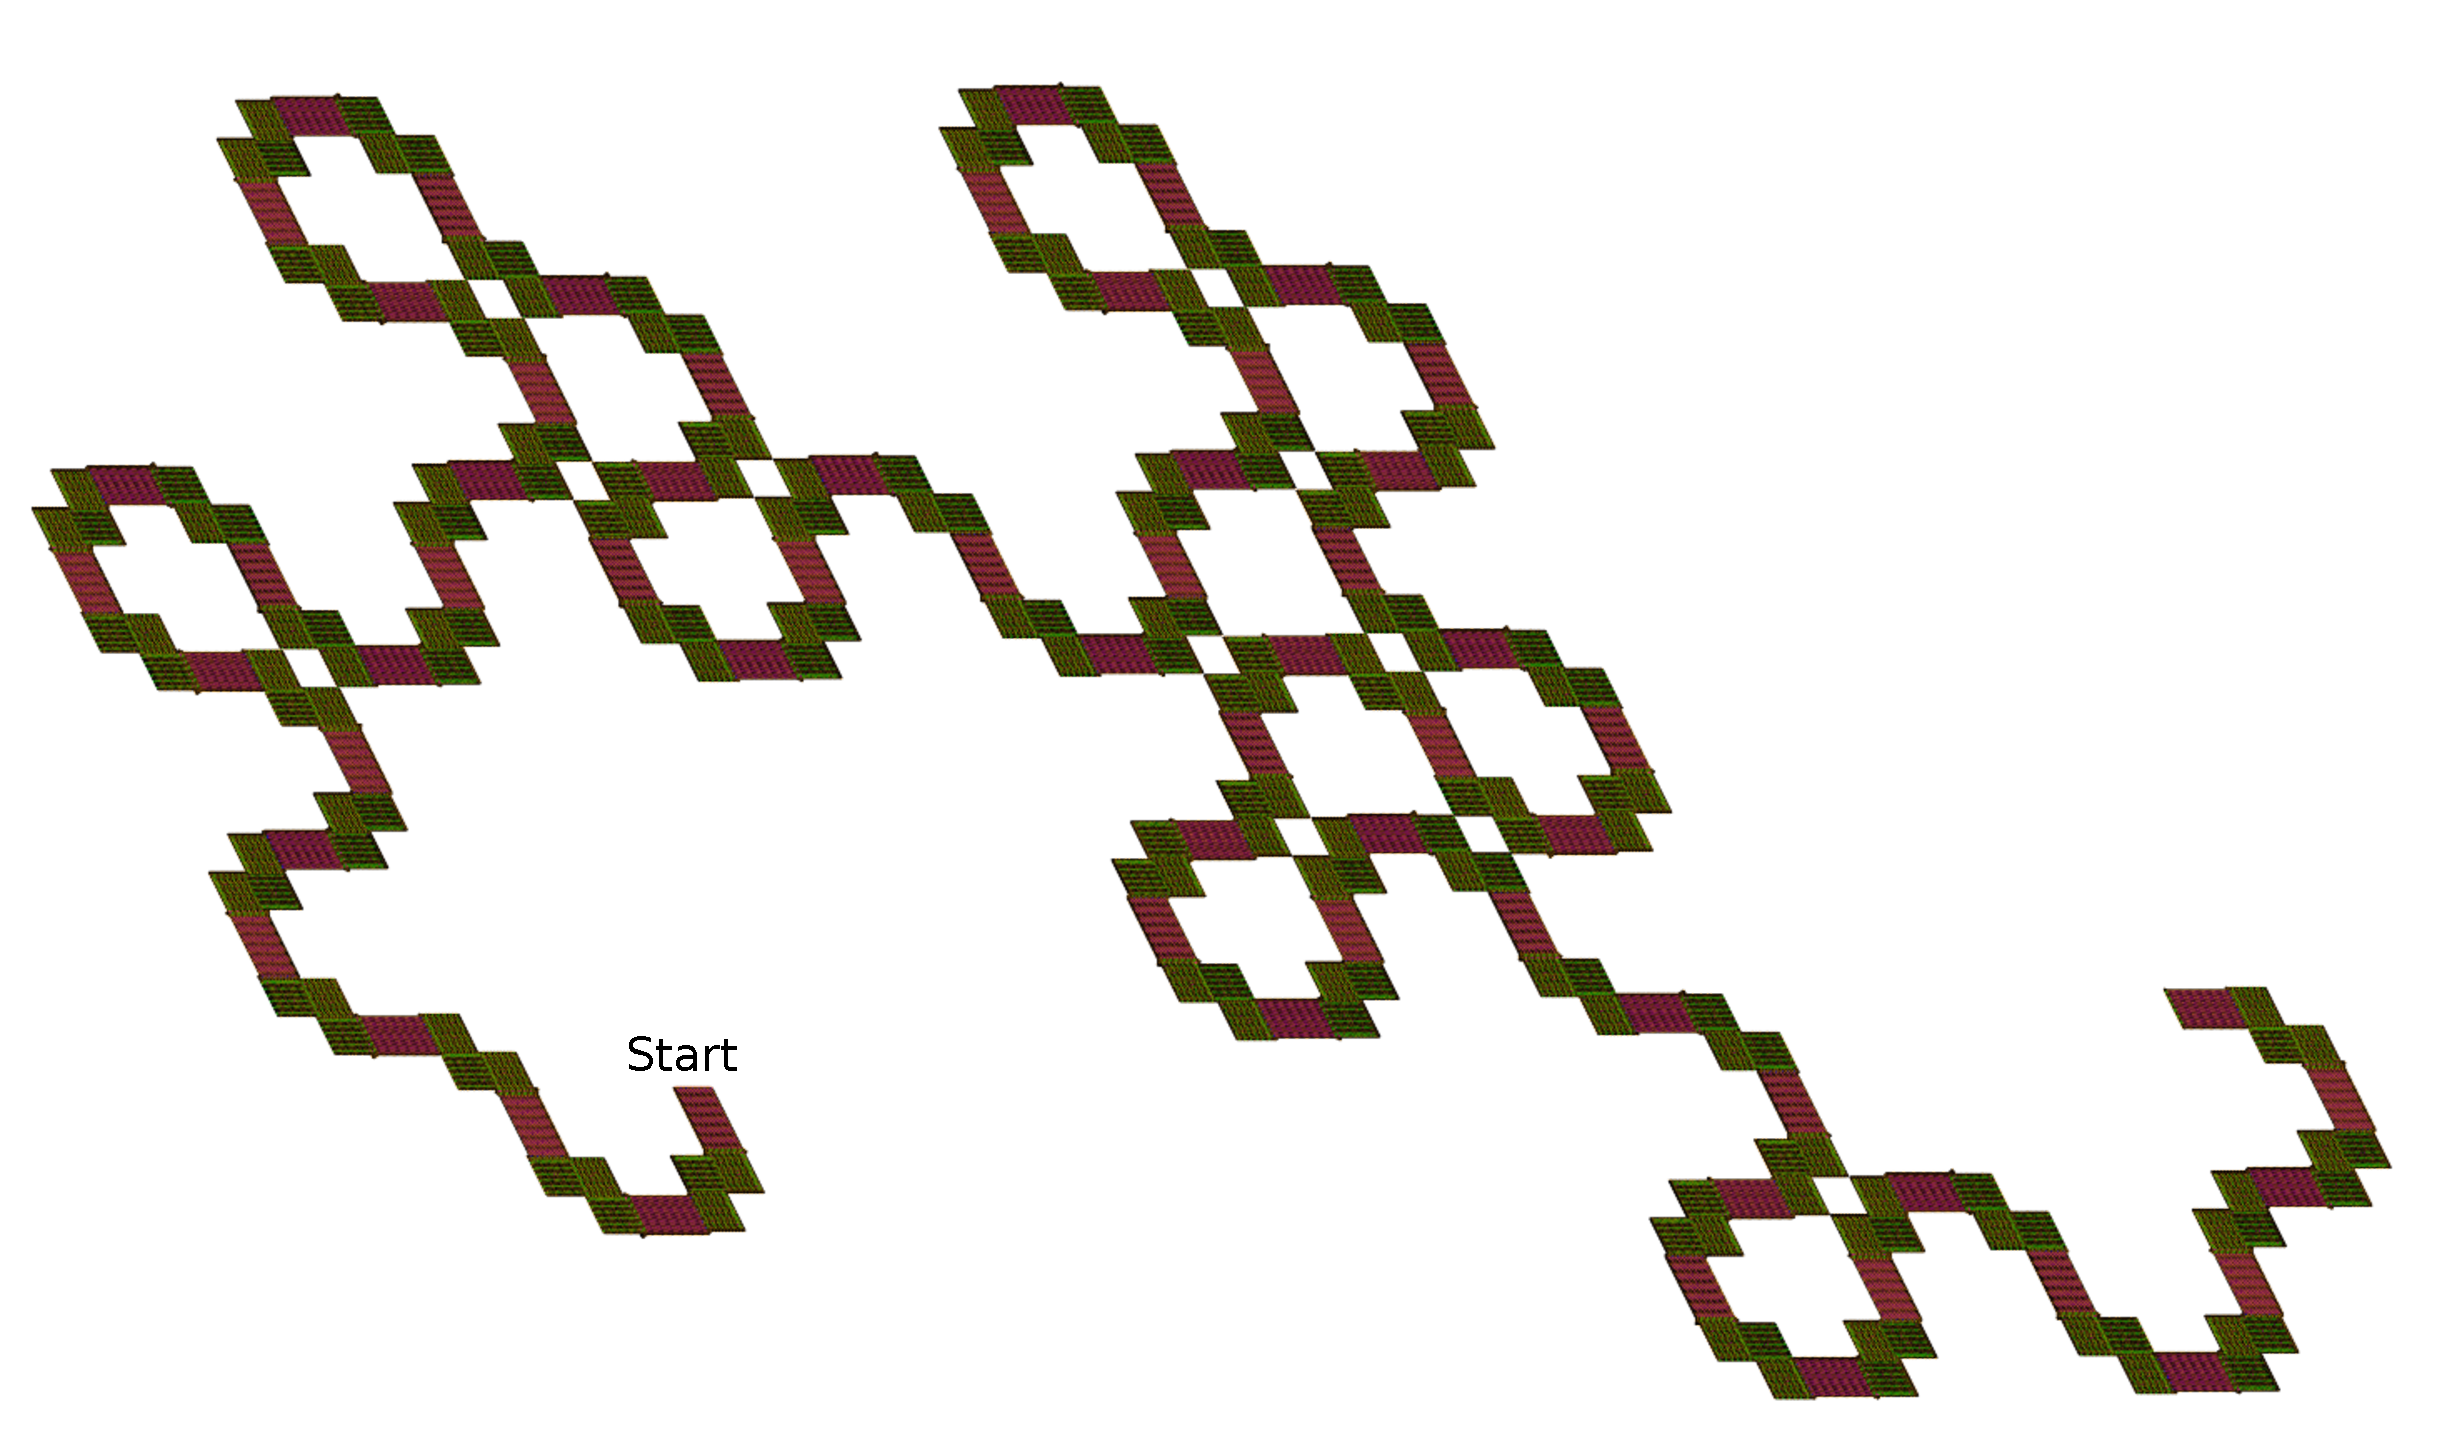
\includegraphics[width=\linewidth]{pic/6bit_heighway.pdf}
\caption{The portion $P[0 .. 62]$ of the Heighway dragon folded by the proposed oritatami system.}
\label{fig:heighway6_oritatami}
\vspace*{-5mm}
\end{wrapfigure}
%\end{figure}

In this paper, we propose a generic design of oritatami system for the algorithmic cotranscriptional folding of an arbitrary finite portion of the Heighway dragon. 
Fig.~\ref{fig:heighway6_oritatami} shows the portion $P[0 .. 62]$ thus folded (the dragon is slanted but this is because the OS operates on the triangular grid). 
The transcript is a repetition of three modules: a catenation of binary counters, DFAO module, and turning module. 
The counter is a technical modification of the one proposed in \cite{GeMeScSe2016}. 
By being fed with carry exactly once, the catenation increments the count $i$ exactly by 1 while folding into a (red) line segment. 
%It folds into one zigzag and increments a given binary number by 1 if carried-in or just propagates the number otherwise. 
%Binary counters fold into zigzags, yielding a (red) line segment of the dragon. 
%The system feeds only the first counter with carry so that the line segment amounts to increment the current count $i$ by 1. 
At the end of the segment comes a DFAO module, which computes the turn direction $P[i]$, reinterprets it properly as A/O, and propagates the count $i$ for the next turning module. 
A (green) L-shaped block is the turning module. 
It is a concatenation of three bit-sequence bifurcators, each of which folds into a rhombus, bifurcates $i$ leftward as well as rightward, and guides further folding according to A/O. 
%We shall implement the DFAO and turning modules and verify them. 

The generic design proves the next theorem (for terminologies, see Sect.~\ref{sect:preliminaries}). 

\begin{theorem}\label{thm:main}
	For any finite portion $P[i..j]$ of the Heighway dragon, there exist an integer $c$ and a deterministic cyclic oritatami system of delay 3 and arity 3 that weakly folds into the $c$-rhombus scaling of $P[i..j]$. 
\end{theorem}

\noindent
A JavaScript program to run this OS is available at {\small {\tt https://wolves13.github.io}}. 

